\documentclass[12pt, letterpaper,spanish]{article}
\usepackage[letterpaper]{geometry}
\usepackage[T1]{fontenc} %para escribir con caracteres utf8 como tildes
\usepackage[utf8]{inputenc} %para escribir con caracteres utf8 como tildes
\usepackage[spanish]{babel} %para escribir con caracteres utf8 como tildes
\usepackage{lmodern} % latin modern font
\usepackage{color}
\usepackage[svgnames]{xcolor} % para hacer enfasis con colores
\usepackage{amssymb}
\usepackage{amsmath}
\usepackage{hyperref}
\usepackage{multirow}
\usepackage{array}
\usepackage{mathtools} % para el modulo
\DeclarePairedDelimiter\abs{\lvert}{\rvert}%
\DeclarePairedDelimiter\norm{\lVert}{\rVert}%
\hypersetup{
	colorlinks=true,
	linkcolor=black,
	filecolor=magenta,      
	urlcolor=cyan,
}

\usepackage{listings}
\lstloadlanguages{Python}
\definecolor{background}{rgb}{0.52, 0.52, 0.51}
\definecolor{keywords}{rgb}{1.0, 0.0, 0.5}
\definecolor{comments}{rgb}{0.75, 0.75, 0.75}
\definecolor{strings}{rgb}{0.91, 0.84, 0.42}
\definecolor{names}{rgb}{0.4, 1.0, 0.0}
\definecolor{white}{rgb}{1.0, 1.0, 1.0}
\definecolor{types}{rgb}{0.13, 0.67, 0.8}
\definecolor{numbers}{rgb}{0.54, 0.17, 0.89}

\lstdefinelanguage{PSharp}{
	keywords={method, include, if, else, elif, while, continue, break, return},
	keywordstyle=\color{keywords}\bfseries,
	ndkeywords={int, void, rider, true, false},
	ndkeywordstyle=\color{types}\bfseries,
	identifierstyle=\color{white},
	sensitive=false,
	emph={print, test, example, Rossi, curves},
	emphstyle=\color{names},
	comment=[l]{//},
	morecomment=[s]{/*}{*/},
	commentstyle=\color{comments}\ttfamily,
	stringstyle=\color{strings}\ttfamily,
	morestring=[b]',
	morestring=[b]"
}

\lstset{
	language=PSharp,
	backgroundcolor=\color{background},
	extendedchars=true,
	basicstyle=\footnotesize\ttfamily,
	showstringspaces=false,
	showspaces=false,
	numbers=left,
	numberstyle=\footnotesize,
	numbersep=9pt,
	tabsize=2,
	breaklines=true,
	showtabs=false,
	captionpos=b
}


\usepackage{amsthm} % para teoremas y lemas
\usepackage{graphicx} % para imagenes
\usepackage{titling} % para el pretitle
\usepackage{clrscode3e} % para pseudocodigos
\usepackage[stable]{footmisc} % para permitir footnotes in los encabezados

%\usepackage[cache=false]{minted} %para representar los codigos necesita config extra
%\renewcommand\theFancyVerbLine{\normalsize\arabic{FancyVerbLine}} % incrementar el tamaño de linenumbers de minted


\newtheorem{theorem}{Teorema}[subsection]
\newtheorem{corollary}{Corolario}[theorem]
\newtheorem{lemma}{Lema}[subsection]
\newtheorem{lemmacorollary}{Corolario}[lemma]
\theoremstyle{definition}
\newtheorem*{definition}{Definición}
\theoremstyle{remark}
\newtheorem*{remark}{Observación}
\renewcommand{\qedsymbol}{$\blacksquare$} % se remplaza el simbolo vacio de final de demostración
\graphicspath{ {./_static/} }

%--------------------------
% NO MODIFICAR ESTE DOCUMENTO
%--------------------------
	
\begin{document}
	
\begin{titlepage}
	\begin{center}
		
\includegraphics[width = 3cm]{escudoUH} 
	\end{center}
	\begin{center}
		Universidad de La Habana \\\vspace{0.2cm} Facultad de Matemática y Computación
	\end{center}
	\centering
	\vspace{1cm} \par
	{\scshape\Large Proyecto de Compilación + Intenteligencia Artificial + Simulación\par}
	\vspace{5mm} \par
	{\scshape\Huge Simulador de un Jefe Técnico de MotoGP\par}
	\vspace{5mm} \par
	\vfill
	{\Large \textbf{Autores:} \par}
	{\large Arnel Sánchez Rodríguez \space Grupo: C312 \par}
	\href{mailto:arnelsanchezrodriguez@gmail.com}{arnelsanchezrodriguez@gmail.com}\par
	\vspace{3mm} \par
	{\large Samuel Efraín Pupo Wong \space Grupo: C312 \par}
	\href{mailto:s.pupo@estudiantes.matcom.uh.cu}{s.pupo@estudiantes.matcom.uh.cu}
	\vspace{3mm} \par
	{\large Darián Ramón Mederos \space Grupo: C312 \par}
	\href{mailto:darianrm24@gmail.com}{darianrm24@gmail.com}
	\vspace{3mm} \par
	\vfill
	{\Large 2021-2022 \par}
\end{titlepage}	
\pagebreak
\tableofcontents
\pagebreak
\section{Motociclismo de Velocidad}
	El motociclismo de velocidad es una modalidad deportiva del motociclismo disputada en circuitos de carreras pavimentados. Las motocicletas que se usan pueden ser prototipos, es decir desarrolladas específicamente para competición, o derivadas de modelos de serie (en general motocicletas deportivas) con modificaciones para aumentar las prestaciones. En el primer grupo entran las que participan en el Campeonato Mundial de Motociclismo, y en el segundo las Superbikes, las Supersport y las Superstock.
	
	Las motocicletas deben presentar una serie de características como son estabilidad, alta velocidad (tanto en recta como en paso por curva), gran aceleración, gran frenada, fácil maniobrabilidad y bajo peso.
	
	\begin{center}
		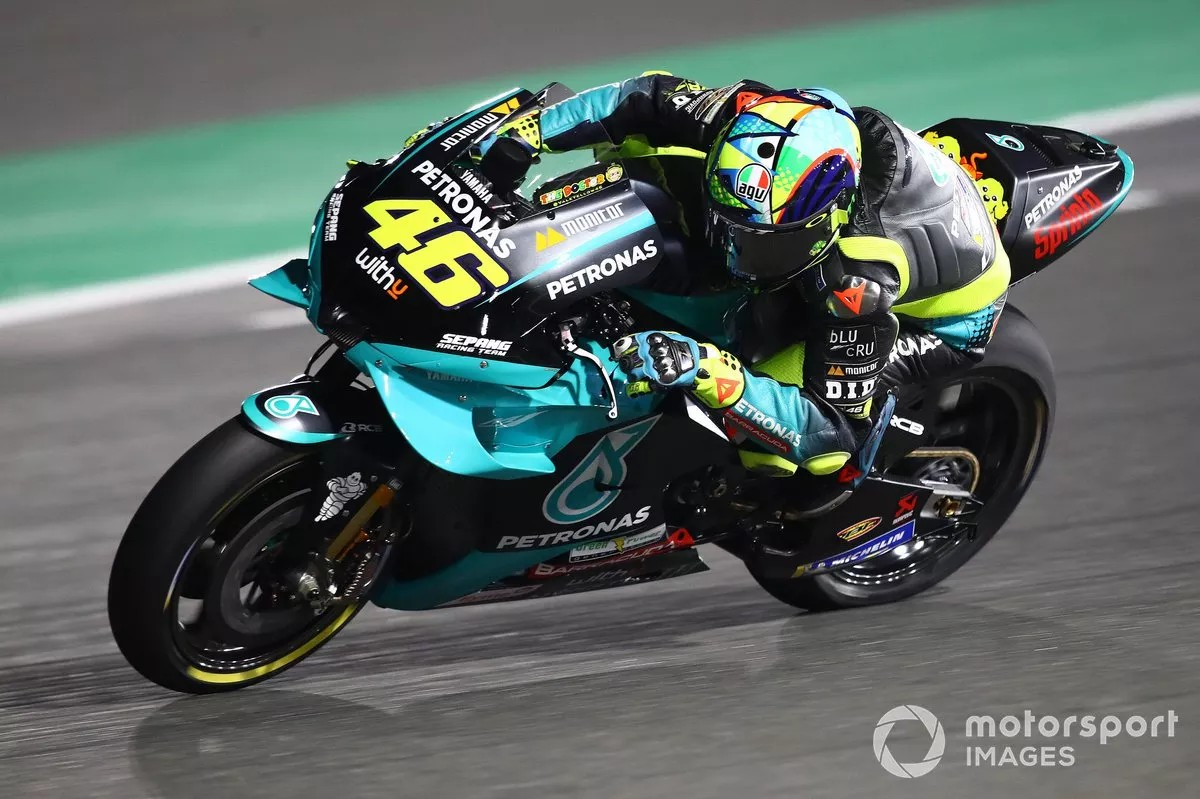
\includegraphics[width = 12cm]{imagen1} 
	\end{center}	
	
\section{Estructura del Paddock}
	El \textbf{Jefe Técnico} de cada estructura se configura como una personalidad de bastante importancia dentro de un box, pues es quién se encarga de dirigir y controlar que todo funcione como un excelente engranaje que gane carreras. De igual importancia es la telemetría dentro de un box en MotoGP. Al fin y al cabo, los \textbf{Ingenieros Telemétricos} son las personas que se encargan de analizar, leer y comprender todos los datos proporcionados por el piloto, así como transmitirselos en boca al protagonista. Se trata de una figura de la que depende mucha de la información acerca de cualquier cambio realizado en la moto o asumir los puntos más fuertes de sus pilotos. Los \textbf{Mecánicos} también desempeñan un papel fundamental a la hora de construir la máquina perfecta.

\section{Pista}
	Se utilizará como referencia el circuito de Misano, Misano World Circuit Marco Simoncelli, autódromo localizado en la fracción de Santa Mónica, comuna de Misano Adriático (provincia de Rímini), región de Emilia-Romaña, Italia. 
	
	\begin{center}
		\includegraphics[width = 12cm]{circuito} 
	\end{center}
	
\section{Definición del Problema}
	Existirán varios pilotos con sus respectivas motos, las cuáles difieren entre sí en cuanto a sus prestaciones. Cada piloto posee sus propias habilidades para circular por curvas y rectas, de acuerdo a ellas es la velocidad que le será posible alcanzar en el tipo de sección. La pista se encuentra influenciada por el accionar del clima, puesto que no es lo mismo el manejo durante un día soleado que bajo la lluvia. Por tanto, el resultado de un piloto se verá condicionado por su moto, su habilidad de conducción y el clima.\par
	Sin embargo, durante la carrera las condiciones pueden variar y el Jefe Técnico será el encargado de señalar los ajustes necesarios que el piloto deberá hacer para mejorar su rendimiento. Dicho intercambio de información se hará al finalizar la vuleta mediante el uso del DSL en el caso que sea el piloto controlado, los demás pilotos se hará la comunicación mediante el uso de la Inateligencia Artificial. \par
	De esta manera, la simulación de la carrera será dinámica, puesto que entre las vueltas podrán existir variaciones provocadas por los ajustes propuestos por el Jefe Técnico.\par
	
\section{Definición del Lenguaje}
	\include{DefiniciónDelLenguaje.tex}
	
\section{Simulación}
	\include{Simulación.tex}

\section{Inteligencia Artificial}
	Como nuestro proyecto se basa en simular una carrera de MotoGP donde hay n corredores, aquellos que no hayan sido diseñados mediante DSL son controlados por IA, el comportamiento de la cual varía a partir de las condiciones del ambiente que lo rodea, las características de su moto y la experiencia del propio piloto.

Para la implementación de la IA se utilizan Sistemas Expertos generados mediante el uso de un procedimiento declarativo/imperativo, apoyándonos en la biblioteca PyKE de Python.

Se emplea como base de conocimiento el conjunto de variables que forman parte de la simulación y que influyen en su desempeño, como:
\begin{itemize}
	\item las características de la moto (velocidad, frenos, chasis)
	\item el estado del clima (soleado, nublado o lluvioso)
	\item la intensidad y el sentido del viento
	\item la humedad y la temperatura del ambiente
	\item la sección de pista que se está corriendo (curva o recta)
	\item la velocidad máxima alcanzable en la sección
	\item las habilidades del piloto (en rectas y curvas)
	\item entre otros
\end{itemize}

\subsection{Configuración de la moto}
	La primera heurística es la encargada de escoger la mejor configuración de la moto. De este modo, atendiendo a las condiciones iniciales de la carrera (que serán los hechos), la IA podrá tomar decisiones atendiendo a las reglas definidas. Al ser declarativas, las determinaciones tomadas se obtendrán mediante match hechos-reglas.
	Los hechos del sistema se presentan mediante una lógica difusa y son procesados para ser analizados:
	%Imagen de hechos

	Las reglas del sistema se formulan del modo:
	%imagen de reglas

	Luego, consultando los resultados obtenidos por las librerías de PyKE, mediante Python de manera imperativa será posible la interacción de la estructura antes expuesta con la simulación de la carrera.
	Atendiendo al ejemplo mostrado de selección de gomas, el sistema declarativo de PyKE devuelve el cálculo de una ecuación:
	$valor_tipo_goma + valor_goma = selección$

	El resultado obtenido se utiliza para generar el tipo de las gomas seleccionadas, mediante el uso de un Enum en Python:
	\begin{lstlisting}[language={Python}, label={Script}]
		class Tires(Enum):
		    Slick_Soft = 0
		    Slick_Medium = 1
		    Slick_Hard = 2
		    Rain_Soft = 3
		    Rain_Medium = 4
	\end{lstlisting}


\subsection{Selección de acciones}
	Una segunda heurística será la encargada de escoger la acción que debe ejecutar el piloto, atendiendo a las condiciones de la carrera:
	\begin{itemize}
		\item aumentar/disminuir/mantener velocidad
		\item doblar
		\item ir a los pits
		\item combinaciones de todas las anteriores
	\end{itemize}
  	(Ejemplo: aumentar velocidad + doblar + ir a los pits)
	En este caso, se utiliza el mismo método expuesto en la configuración de la moto: declarativo/imperativo con el uso de PyKE.
	Se analizan los parámetros de velocidad, sección de la pista y estado del clima:


	Y se decide tomándolos en cuenta:


	Asimismo, se calcula mediante una ecuación el valor de la decisión tomada:
	$acción_velocidad + doblar + pits = acción$

	\begin{lstlisting}[language={Python}, label={Script}]
		class AgentActions(Enum):
			SpeedUp = 0
			KeepSpeed = 1
			Brake = 2
			SpeedUp_Turn = 3
			KeepSpeed_Turn = 4
			Brake_Turn = 5
			SpeedUp_Pits = 6
			KeepSpeed_Pits = 7
			Brake_Pits = 8
			SpeedUp_Turn_Pits = 9
			KeepSpeed_Turn_Pits = 10
			Brake_Turn_Pits = 11
	\end{lstlisting}

\subsection{Selección de la aceleración}
	Una tercera heurística es la encargada de escoger la mejor aceleración en una sección dada de la pista, con el objetivo de alcanzar la mayor velocidad posible sin causar un accidente que obligue a abandonar la carrera. 
	Primeramente, se calcula la aceleración máxima alcanzable, tomando en cuenta que no se exceda la velocidad máxima admitida por la moto y la sección que se recorre.
	$$a_max=(V_max^{2}-V^{2})/(2*X)$$
	Luego, se establece un sistema de penalizaciones que disminuyen dicha aceleración si no se poseen las condiciones óptimas del ambiente (clima, humedad, temperatura) y del piloto (destreza en curvas y rectas).
	El resultado obtenido es incorporado a la simulación para continuar la carrera. De su valor depende mucho si el piloto obtiene un buen tiempo o sufre un accidente que lo saque de la competencia.


\end{document}

